\documentclass{article}

% Language setting
% Replace `english' \begin{figure}[H]
\centering
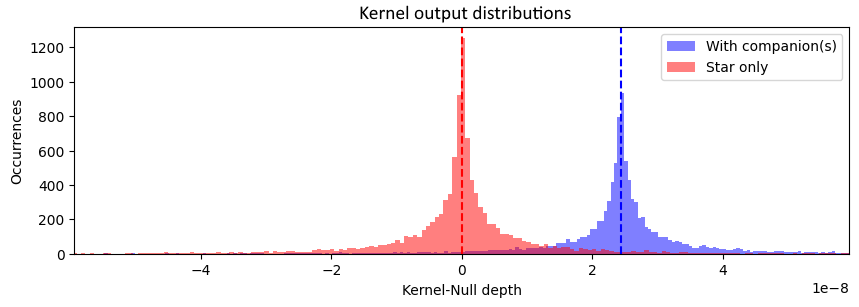
\includegraphics[width=\linewidth]{img/output_distribution.png}
\caption{Example of kernel nulling depth $$
\begin{cases}
H_0 : D_m = |\tilde{n}|\\
H_1 : D_m =  | \alpha S_p + \tilde{n} |
\end{cases}
$$

Surprisingly, the median proves to be a very efficient test statistic in this context (figure \ref{fig:roc}), surpassing many more sophisticated tests like those listed in section \ref{sec:other_tests}. However, it requires a large number of samples to be effective, which can be a disadvantage in situations where observation time is limited.tions for hypotheses $\mathcal{H}_0$ (star alone) and $\mathcal{H}_1$ (with companion). This example scenario is heavily exaggerated with a companion having low contrast to induce a significant distribution shift. In practice, the two distributions are generally much closer and difficult to distinguish.\dm{Cf texte; aussi prends l'habitude d'être ultra-spécifique, c'est un papier scientifique. Là tu es bcp trop vague : "low contrast" (c'est quoi low ?) "much closer" (=?..)}.}
\label{fig:distribution}
\end{figure}.g. `spanish' to change the document language
\usepackage[en
glish]{babel}

% Custom packages
\usepackage{color,soul} % For highlighting text
\usepackage{float} % For controlling figure placement ([H] option)
\usepackage{amsmath}
\usepackage{amssymb} % For mathematical symbols such as \lessgtr
\DeclareMathOperator*{\argmax}{arg\,max}
\DeclareMathOperator*{\argmin}{arg\,min}

% Set page size and margins
% Replace `letterpaper' with `a4paper' for UK/EU standard size
\usepackage[letterpaper,top=2cm,bottom=2cm,left=3cm,right=3cm,marginparwidth=1.75cm]{geometry}

% Useful packages
\usepackage{graphicx}
\usepackage[colorlinks=true, allcolors=blue]{hyperref}

\definecolor{mulberry}{rgb}{0.77, 0.29, 0.55}
\newcommand{\dm}[1]{{\color{mulberry} #1}}

\newcommand{\mi}{\mathrm{i}}

\title{Statistical analysis of Kernel-Nulling output distributions for high-contrast exoplanet detection in VLTI and LIFE configurations}

\author{Vincent Foriel,
        David Mary,
        Frantz Martinache
       }

\begin{document}

\maketitle

\begin{abstract}
\begin{abstract}
Kernel-Nulling interferometry represents a promising approach for direct detection of exoplanets. This technique generates characteristic intensity distributions depending on the presence or absence of a planetary companion. Statistical analysis of these distributions is essential for robust planet detection. We develop and compare several statistical tests to efficiently discriminate between hypotheses $\mathcal{H}_0$ (star alone) and $\mathcal{H}_1$ (star-planet system). We analyze the performance of different test statistics to evaluate the relevance of each according to the nature of the available data. We perform numerical simulations for three instrumental scenarios: ground-based VLTI configurations and the LIFE space mission, as well as a fictional scenario consisting of placing the VLTI in space to isolate performance losses caused by the atmosphere. For each scenario, we generate datasets under both hypotheses $\mathcal{H}_0$ and $\mathcal{H}_1$, taking into account specific instrumental parameters and noise levels. We evaluate test performance using ROC curves and P-value analysis. \hl{Add results}. This statistical analysis, currently applied to simulated data, paves the way for robust detection of high-contrast exoplanets using kernel-nulling interferometry.
\end{abstract}
\end{abstract}

\dm{OK résumé de mes coms détailles ci-dessous : le plus gros boulot à faire pour l'itération suivante c'est : \\
- en intro : biblio : recenser, comparer, contraster pour mettre en évidence l'originalité du papier\\
- en intro : justification de l'intérêt scientifique du papier (/exoplanètes, VLTI, LIFE) et de son scope (portée attendu des simus ?) \\
- Sec. 2 étude statistique plus poussée des différents régimes, types de distribution, influence des paramètres, classement et présentation des résultats pour justifier la section d'après (les tests mis en opuvre)\\
- Sec. 3 : La formalisation rigoureuse des tests, classement, formules analytiques \\
- Sec. 4 : Etude comparative des performances dans les résultats }

%==============================================================================
\section{Introduction}
%==============================================================================

Direct imaging of exoplanets remains one of the major challenges in modern astronomy, requiring techniques capable of overcoming contrast constraints (beyond $10^{-8}$ to enable detection of Earth-like exoplanets) and angular separation requirements (on the order of milli-arcseconds). Nulling interferometry, initially proposed by \cite{Bracewell1979}, uses destructive interference to suppress the on-axis source (stellar light) while preserving off-axis sources (planetary signals), thus addressing both angular resolution and contrast challenges.

Kernel-Nulling (\cite{Martinache2018}) improves this approach by focusing on the difference between pairs of symmetric beam combinations that are robust to first-order phase aberrations (\cite{Martinache2018}). Due to various perturbation sources, the output of the nulling operation - as well as the Kernel-Nulling operation - is a statistical distribution of intensities. This distribution is influenced by various instrumental parameters such as input co-phasing errors, amplitude errors, number of frames, sky background or even other sources of undesirable light such as background stars (\cite{Hanot2011}, \cite{Cvetojevic2022}). The presence of a companion induces a systematic co-phasing error that cannot be approximated by a first-order perturbation, leading to a global shift in the Kernel-Null output distributions. This results in distinct statistical distributions for the kernel-null output depending on whether a companion is present or not (see Fig. \ref{fig:distribution}). In realistic scenarios, the shift induced by the companion's presence is small compared to the dispersion due to various perturbation sources, making the $\mathcal{H}_0$ and $\mathcal{H}_1$ distributions difficult to distinguish. The number of frames used in the simulation also affects the spread and smoothness of distributions. A detailed analysis of the influence of these parameters and resulting distribution families is provided in Sec. \ref{sec:distribution_analysis}. However, these distributions do not follow standard probability laws, and their analytical form is unknown a priori. This makes the discrimination problem difficult, particularly when the companion contrast is high and the distributions overlap significantly.

The analysis of these distributions therefore requires appropriate statistical tools to efficiently discriminate between the two hypotheses: $\mathcal{H}_0$ (star alone) and $\mathcal{H}_1$ (star-planet system). In this work, we develop and compare several statistical tests to optimize exoplanet detection using Kernel-Nulling.

\dm{Il manque :\\
- Une biblio minutieuse de ce pb : mettre en évidence des différence entre des distributions dans un contexte exoplanètes, et plus généralement astro, ça existe où ? Comment les gens font ? Qu'est-ce que tu prends d'eux et qu'est ce que tu vas apporter de nouveau ? Quelles différences entre les problématiques connexes que tu as trouvées et la tienne ? Expliquer points communs et différences.\\
- Justification de l'intérêt de ce papier par rapport aux instruments visés / VLTI et LIFE. Faire un topo sur VLTI et lIFE par rapport à la détection d'exoplanètes. Puis décrire comment l'approche kernel-nulling se compare aux autres approches de détection exoplanètes (pros/cons) ? Et enfin sur l'approche quel est le statut des méthodes prévues ? (en gros : on ne sait pas vraiment faire, ton papier est très important pour poser des algos. Mais attention contraster par rapport aux travaux de Hanot \& co que je t'ai fait suivre par mail; et il y en a probablement d'autres.)\\ 
- plan du papier}

\begin{figure}[H]
\centering
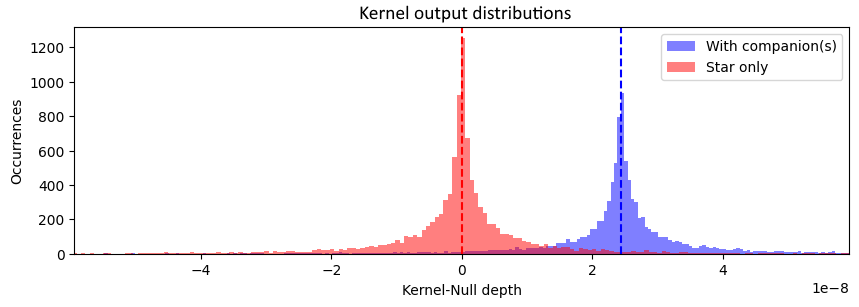
\includegraphics[width=\linewidth]{img/output_distribution.png}
\caption{Exemple de distributions de profondeur d'annulation par noyau pour les hypothèses $\mathcal{H}_0$ (étoile seule) et $\mathcal{H}_1$ (avec compagnon). Ce scénario d'exemple est fortement exagéré avec un compagnon qui a un faible contraste afin d'induire un décalage significatif de la distribution. En pratique, les deux distributions sont généralement beaucoup plus proches et difficiles à distinguer.\dm{Cf texte; aussi prends l'habitude d'être ultra-spécifique, c'est un papier scientifique. Là tu es bcp trop vague : "low contrast" (c'est quoi low ?) "much closer" (=?..)}.}
\label{fig:distribution}
\end{figure}



%==============================================================================
\section{Methodology}
%==============================================================================



%------------------------------------------------------------------------------
\subsection{Data generation}

In this study, we consider three instrumental scenarios corresponding to realistic configurations of interferometers dedicated to exoplanet detection, each with its own technological constraints and expected performance.

\textbf{The Very Large Telescope Interferometer (VLTI)} represents the current state of the art in ground-based interferometry. This instrument combines light from four 8-meter diameter unit telescopes (UT), arranged in an irregular configuration with a maximum baseline of 130 meters. This configuration allows achieving a theoretical angular resolution on the order of 1 milli-arcsecond at $1.55\mu$m, the optimal wavelength for observation in the H-band of the near infrared. However, terrestrial atmospheric conditions introduce significant phase perturbations: despite adaptive optics systems and real-time co-phasing correction, residual co-phasing error remains on the order of 100 nm RMS. This value, while representing remarkable performance for a ground-based instrument, nevertheless constitutes a fundamental limitation for very high-contrast exoplanet detection, where phase stability must be maintained at extreme levels over long integration times.

\textbf{The LIFE space mission (Large Interferometer For Exoplanets)} embodies the future of interferometry dedicated to exoplanet detection. This mission plans the orbital deployment of four 2-meter diameter telescopes arranged in a rectangular formation with a baseline that can reach 600 meters. The space environment offers decisive advantages: the absence of atmosphere eliminates turbulence and allows unprecedented phase control precision, with co-phasing errors reduced to 1 nm RMS. This exceptional stability, coupled with the observation wavelength of $4\mu$m in the thermal infrared, opens the way to direct detection of Earth-like exoplanets and spectroscopy of their atmospheres for the search for biosignatures.

\textbf{The SVLTI scenario (Space VLTI)} constitutes a theoretical case study allowing isolation of the specific impact of Earth's atmosphere on detection performance. By transposing the exact VLTI configuration (four 8-meter telescopes, irregular arrangement, 130-meter baseline) into the space environment, we maintain the same observation wavelength ($1.55\mu$m) while benefiting from space co-phasing stability (1 nm RMS). This hybrid configuration allows direct comparative analysis: by comparing VLTI/SVLTI performance, we precisely quantify the degradation caused by atmospheric perturbations, while the SVLTI/LIFE comparison reveals the impact of instrumental architecture (telescope size, wavelength, geometry) on detection efficiency.

In summary, we have:
\begin{table}[H]
\centering
\begin{tabular}{|l|c|c|c|}
\hline
\textbf{Parameter} & \textbf{VLTI} & \textbf{LIFE} & \textbf{SVLTI} \\
\hline
Number of telescopes & 4 & 4 & 4 \\
Telescope diameter & 8 m & 2 m & 8 \\
Configuration & Irregular & Regular (rectangular) & Irregular \\
Maximum baseline & 130 m & 600 m & 130 \\
Operating environment & Ground & Space & Space \\
Wavelength & $1.55\mu$m & $4\mu$m & $1.55\mu$m \\
Co-phasing error (RMS) & 100 nm & 1 nm & 1 nm \\
\hline
\end{tabular}
\caption{Instrumental parameters for the three scenarios considered in this study.}
\label{tab:scenarios}
\end{table}

For each of the simulations performed, we consider a zero-magnitude primary source (Vega-type star) with a single hypothetical companion whose position and contrast are fixed. This work being interested in the theoretical limits achievable in terms of detection capability, we work under the assumption of a thermally stable environment and an ideal camera, i.e., without readout noise or background noise. We simulate series of 1-second acquisitions integrating the effects of residual co-phasing errors (atmospheric perturbations and intrinsic optical path difference of the system) and photon noise. For each scenario, we generate datasets under both hypotheses $\mathcal{H}_0$ (star alone) and $\mathcal{H}_1$ (star-planet system), taking into account specific instrumental parameters and noise levels for each case.



%------------------------------------------------------------------------------
\subsection{Statistical tests and likelihood ratio}

To discriminate between hypotheses $\mathcal{H}_0$ (star alone) and $\mathcal{H}_1$ (star-planet system), several test statistics are used in our simulations:

\begin{itemize}
    \item \textbf{Mean} : $T(u) = |\mathrm{mean}(u)|$
    \item \textbf{Median} : $T(u) = |\mathrm{median}(u)|$
    \item \textbf{Kolmogorov-Smirnov} : $T(u, v) = |D_{KS}(u, v)|$ where $D_{KS}$ is the KS statistic between two samples
    \item \textbf{Flattening} : $T(u) = \sum_i |u_i - \mathrm{median}(u)|$
\end{itemize}

Each test allows quantifying the difference between distributions arising from the two hypotheses. Performance is evaluated via ROC curves and P-value analysis.

For each scenario, datasets are generated under both hypotheses $\mathcal{H}_0$ (star alone) and $\mathcal{H}_1$ (star-planet system), taking into account specific instrumental parameters and noise levels for each case. The Kernel-Nulling operation is assumed to be ideal.\dm{Je pense qu'il faut prévoir un appendice où tu résumes le principe de kernel-nulling pour que le lecteur te suive; qu'il comprenne ce que signifie faire une operaiton de kernel nulling en pratique, et lister tous les défauts qui font que ça ne peut pas être idéal. Il faut aussi différencier une operation de kernel null idéale et l'absence de bruit à la fin. Bien expliquer ce que capturent tes simulations et les fluctuations qui créent les distributions montrées en Fig. 1.}



%------------------------------------------------------------------------------
\subsection{Analyse des distributions}  \label{sec:distribution_analysis}

Avant de tenter de discriminer entre les hypothèses $\mathcal{H}_0$ et $\mathcal{H}_1$, il est essentiel d'étudier les distributions obtenues pour identifier les caractéristiques qui pourraient faciliter leur analyse. À cette fin, nous comparons les distributions simulées à différentes lois de probabilité conventionnelles, en observant notamment leur symétrie et leur forme générale.

Nous trouvons qu'aucune loi conventionnelle ne correspond parfaitement aux distributions observées. \dm{$<=$ Ca c'est une conclusion. Pour que cette phrase ait du poids, il faut présenter une analyse détaillée de ces distributions (comme le titre le suggère) : montrer comment les variations combinées de tous les paramètres importants mènent à des distributions différentes. Identifier et montrer tous les différents régimes de paramètres menant à des familles de distributions différentes. Lister aussi tous les pramètres qui vont entrer en compte dans les perfs de détections : contraste et position du compagnon, longueur d'onde donc, nombre de trames, puissance des erreurs de phase, D telescope,... tu peux faire une table. Une étude scientifique est vraiment une étude scientifique : on essaie d'être exhaustif dans l'analyse, et ensuite de faire une synthèse quantifiée et bien rangée qui reflète clairement tous les cas pour le lecteur. Le but est d'en faire un expert en lui donnant toutes les infos pour qu'ils le deviennent en lisant le papier, et puisse reproduire les résultats s'il le souhaite (c'est le propre de la démarche scientifique, éviter d'être juste déclaratif ce qui revient à proposer des arguments d'autorité; préférer systématiquement être aussi précis que possible et donner toutes les infos, ce qui revient à proposer des arguments d'expertise.} Parmi les lois testées, la distribution de Cauchy semble \dm{c'est faible et pas quantifié, et vu la fig.2 ça ne colle pas comme tu le dis} offrir un ajustement relativement satisfaisant (Fig. \ref{fig:fits}), bien que non parfait, en particulier sur les queues lorsque le nombre d'échantillons est élevé.

Cette observation guide le choix des tests statistiques à privilégier, en particulier ceux efficaces pour détecter des décalages dans les distributions symétriques.\dm{Justifier théoriquement et/ou empiriquement (via l'optique et le ssimus) si les distribution doivent être symétriques. Ajouter éveutellement des acquisitions de frames sur banc pour appuyer à un moment ces hypothèses. } De plus, cela suggère que l'ajustement de données en minimisant \dm{$<=$ data fitting of what ? Pas le fit de d'une distribution empirique par une autre en tout cas... on en discutera. } l'erreur quadratique moyenne (MSE) ne sera très probablement pas très efficace en raison des queues lourdes de la distribution. Au lieu de cela, nous devrions utiliser une fonction de coût dérivée de la loi de Cauchy, qui est plus robuste aux valeurs aberrantes :\dm{Non je pense que la fin de la section n'est pas bonne.}
\begin{equation}
    \text{Cost}(x, y) = \sum_i \log \left( 1 + \left( y_i - s(x_i )\right)^2 \right)
\end{equation}

\begin{figure}[H]
\centering
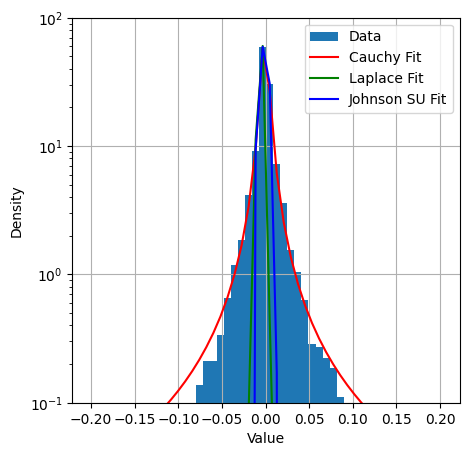
\includegraphics[width=6cm]{img/fits.png}
\caption{Ajustement des lois de probabilité conventionnelles aux distributions simulées. Le package Python Fitter a été utilisé pour effectuer l'ajustement de la plupart des lois usuelles. Cette figure montre l'ajustement des trois lois les plus pertinentes que le package a identifiées.}
\label{fig:fits}
\end{figure}



%------------------------------------------------------------------------------
\subsection{Implemented statistical tests}

In the presence of a companion (hypothesis $\mathcal{H}_1$), the Kernel-Nulling output distribution is modified compared to the star-alone case (hypothesis $\mathcal{H}_0$) as shown in figure \ref{fig:distribution}.

This modification manifests primarily as a distribution shift, although other changes in distribution shape may also occur. Depending on conditions, it is for example possible to observe a flattening of the distribution. To effectively detect the presence of a companion, we have implemented and evaluated several statistical tests, each being sensitive to different aspects of the distributions.

%~~~~~~~~~~~~~~~~~~~~~~~~~~~~~~~~~~~~~~~~~~~~~~~~~~~~~~~~~~~~~~~~~~~~~~~~~~~~~~
\subsubsection{Mean}

The most natural test to perform under these conditions consists of comparing the mean to a threshold. Given that the planet can induce a distribution shift in both directions, we use the absolute value of the mean.

$$
D_{M} = \left|\frac{1}{N}\sum_{i=1}^N x_i \right| \stackrel{H_1}{\underset{H_0}{\gtrless}} \xi
$$

Indeed, under hypothesis $\mathcal{H}_0$, the mean should be close to zero, equivalent to the noise mean $\bar{n}$, while under $\mathcal{H}_1$, it will be shifted according to the planet signal $S_p$ and its transmission $\alpha$ within the system.

$$
\begin{cases}
H_0 : D_M = |\bar{n}|\\
H_1 : D_M =  |\alpha S_p + \bar{n}|
\end{cases}
$$

In practice, we observe that the mean is here a particularly unreliable test statistic (figure \ref{fig:roc}). Indeed, the latter is sensitive to extreme values, yet the considered distributions have heavy tails.

%~~~~~~~~~~~~~~~~~~~~~~~~~~~~~~~~~~~~~~~~~~~~~~~~~~~~~~~~~~~~~~~~~~~~~~~~~~~~~~
\subsubsection{Median}
Another natural test statistic in this context is the median, which is more robust to extreme values than the mean. The median is defined as the central value of a sorted dataset. For a dataset $x_1, x_2, \ldots, x_N$ sorted in ascending order, the median is then the value of the central element if $N$ is odd, or the mean of the two central elements if $N$ is even. As with the mean, we use the absolute value of the median to capture shifts in both directions which we then compare to a threshold.

$$
D_m = 
\begin{cases}
\left| x_{\frac{N+1}{2}} \right| & \text{if }N\text{ is odd} \\

\left| \frac{x_{\frac{N}{2}} + x_{\frac{N+1}{2}}}{2} \right|  & \text{if }N\text{ is even}
\end{cases}
\quad\stackrel{H_1}{\underset{H_0}{\gtrless}} \xi
$$

Very analogously, under hypothesis $\mathcal{H}_0$, the median should be close to zero, equivalent to the noise median $\tilde{n}$, while under $\mathcal{H}_1$, it will be shifted according to the planet signal $S_p$ and its transmission $\alpha$ within the system.

$$
\begin{cases}
H_0 : D_m = |\tilde{n}|\\
H_1 : D_m =  | \alpha S_p + \tilde{n} |
\end{cases}
$$

Surprenament, la médiane s'avère être une statistique de test très performante dans ce contexte (figure \ref{fig:roc}), surpassant bon nombre de tests plus sophistiqués comme ceux listés dans la section \ref{sec:other_tests}. Cependant, elle necessite un grand nombre d'échantillons pour être efficace, ce qui peut être un inconvénient dans des situations où le temps d'observation est limité.

%~~~~~~~~~~~~~~~~~~~~~~~~~~~~~~~~~~~~~~~~~~~~~~~~~~~~~~~~~~~~~~~~~~~~~~~~~~~~~~
\subsubsection{Kolmogorov-Smirnov}

The Kolmogorov-Smirnov (KS) test is a non-parametric test that compares two empirical distributions. It is particularly useful when distributions do not follow a known probability law. The KS test statistic is defined as the maximum distance between the cumulative distribution functions (CDF) of the two samples.

$$
D_{KS} = \sup_x |F_1(x) - F_2(x)| \stackrel{H_1}{\underset{H_0}{\gtrless}} \xi
$$

where $F_1(x)$ and $F_2(x)$ are the empirical CDFs of the two samples. The KS test is sensitive to global differences between distributions, including shifts, dispersion changes, and shape differences.

Under hypothesis $\mathcal{H}_0$, both samples come from the same distribution, while under $\mathcal{H}_1$, they come from different distributions. Thus, under $\mathcal{H}_0$, we expect $D_{KS}$ to be small, proportional to the quadratic combination of noises, while under $\mathcal{H}_1$, $D_{KS}$ will be larger due to deformations induced by the companion's presence.

$$
\begin{cases}
H_0 : D_{KS} \approx |\sqrt{2}\bar{n}|\\
H_1 : D_{KS} \approx |\sqrt{2}\bar{n} + K(S_p)|
\end{cases}
$$

Where $K(S_p)$ is an increasing function of the planet signal $S_p$ that depends on how the distribution is modified by the presence of $S_p$. In practice, the KS test proves to be a robust and efficient test statistic in this context (figure \ref{fig:roc}), although it also requires a large number of samples.



%~~~~~~~~~~~~~~~~~~~~~~~~~~~~~~~~~~~~~~~~~~~~~~~~~~~~~~~~~~~~~~~~~~~~~~~~~~~~~~
\subsubsection{Flattening}

After studying the distribution shift via median and mean, we investigated the flattening effect we could observe in certain configurations. For this, we defined a test statistic we call "flattening", which measures the mean of absolute deviations between each sample and the sample median.

$$
D_f = \frac 1 N \sum_{i=1}^N |x_i - \tilde{x}| \stackrel{H_1}{\underset{H_0}{\gtrless}} \xi
$$

where $\tilde{x}$ is the sample median. Under hypothesis $\mathcal{H}_0$, we expect $D_f$ to be proportional to the noise dispersion, while under $\mathcal{H}_1$, $D_f$ will be modified according to how the distribution is flattened by the companion's presence.

$$
\begin{cases}
H_0 : D_f = \overline{|n_i - \tilde{n}|}\\
H_1 : D_f = \overline{|n_i - \tilde{n}|} \cdot F(S_p)
\end{cases}
$$

Where $F(S_p)$ is an increasing function of the planet signal $S_p$ that depends on how the distribution is flattened by the presence of $S_p$, with $F(0)=1$. The flattening test alone is not intended to be a very efficient test statistic (figure \ref{fig:roc}), but it highlights the fact that flattening is a real effect that can be exploited in addition to other test statistics and which notably motivated the creation of the following test statistic.

%~~~~~~~~~~~~~~~~~~~~~~~~~~~~~~~~~~~~~~~~~~~~~~~~~~~~~~~~~~~~~~~~~~~~~~~~~~~~~~
\subsubsection{Median of Absolute Values}

This statistic measures the median of absolute values of samples, offering a robust measure of both a shift and flattening of the distribution.

$$
D_{MAV} = \text{median}(|x_i|) \stackrel{H_1}{\underset{H_0}{\gtrless}} \xi
$$

Under hypothesis $\mathcal{H}_0$, without flattening or shift, we expect $D_{MAV}$ to be close to the median of absolute noise values, while under $\mathcal{H}_1$, we will recover not only the shift effect present in the median, but also the flattening effect present in the flattening test.

$$
\begin{cases}
H_0 : D_{MAV} = \text{median}(|\mathbf{n}|)\\
H_1 : D_{MAV} = \text{median}(|\mathbf{n} \cdot F(S_p) + \alpha S_p|)
\end{cases}
$$

Where $F(S_p)$ is the same flattening function as in the flattening test. This test statistic proves to be one of the most efficient with numerically obtained distributions (figure \ref{fig:roc}).

%~~~~~~~~~~~~~~~~~~~~~~~~~~~~~~~~~~~~~~~~~~~~~~~~~~~~~~~~~~~~~~~~~~~~~~~~~~~~~~
\subsubsection{Other tests considered}\label{sec:other_tests}
We also explored other statistical tests, notably:
\begin{itemize}
    \item Cramér-von Mises test
    \item Wilcoxon-Mann-Whitney test
    \item Anderson-Darling test
    \item Brunner-Munzel test
\end{itemize}

However, these tests did not show satisfactory performance in our specific context and were therefore not included in the detailed analyses presented in this paper.



\dm{Il manque aussi une 3eme approche  ici qui est un GLR : utliser le modèle direct pour calculer la vraisemblance des données selon la position du compagnon; le GLR cherche alors à maximiser la position du compagnon. C'est les formules que j'avais mises au tableau dans mon bureau et la photo est sur discord. On en re-dicte aussi je sais que ça t'avait fait gamberger. C'est important parce que ce test permet la généralisation à plusieurs kernels. \\
D'ailleurs, il faut que tu parles de ça avant de présenter les tests : tu es en seul kernel jusqu'ici. Et il faudra ajouter  une section : Generalisation des tests considérées à plusiers kernels et/ou poses (= comment les stat de tests monokernel-obs peuvent se combiner).}



%--------------------------------------------------------------------
\subsection{Likelihood Ratio}
The likelihood ratio (LR) test consists of comparing the probability of observing the data under each hypothesis:
\begin{equation}
    \Lambda(x) = \frac{p(x;\mathcal{H}_1)}{p(x;\mathcal{H}_0)}
\end{equation}
where $p(x;\mathcal{H}_i)$ is the probability density of data $x$ under hypothesis $\mathcal{H}_i$. This test is optimal in the Neyman-Pearson sense for minimizing the probability of error for a given false alarm rate. However, it requires analytical knowledge of distributions under each hypothesis, which is not the case in our context as we discussed in section \ref{sec:distribution_analysis}. Among the usual probability laws, we observed that our distributions resembled Cauchy or Laplace laws \ref{fig:fits}, without perfectly fitting them.

 To compare the previous statistical tests to this optimal test, we propose an approach based on parametric model fitting, corresponding to the cited laws, to simulated distributions. We thus assume that the data follow a known probability law and that all statistics of these distributions are comparable to those of simulated data, thus not significantly affecting the performance of different tests.

Let us first consider the classical case where, under each hypothesis, the distribution is Gaussian with mean $\mu_i$ and variance $\sigma_i^2$:
\begin{equation}
    p(x|\mathcal{H}_i) = \frac{1}{\sqrt{2\pi\sigma_i^2}} \exp\left(-\frac{(x-\mu_i)^2}{2\sigma_i^2}\right)
\end{equation}
For $N$ independent observations $\mathbf{x} = \{x_1, x_2, \ldots, x_N\}$, the total likelihood under each hypothesis is the product of individual likelihoods:
\begin{equation}
    p(\mathbf{x};\mathcal{H}_i) = \prod_{j=1}^N p(x_j;\mathcal{H}_i)
\end{equation}
The likelihood ratio is then written:
\begin{align}
    \Lambda(\mathbf{x}) &= \frac{p(\mathbf{x};\mathcal{H}_1)}{p(\mathbf{x};\mathcal{H}_0)} \\
    &= \prod_{j=1}^N \frac{p(x_j;\mathcal{H}_1)}{p(x_j;\mathcal{H}_0)} \\
    &= \left(\frac{\sigma_0}{\sigma_1}\right)^N \exp\left( \sum_{j=1}^N \left[ \frac{(x_j-\mu_0)^2}{2\sigma_0^2} - \frac{(x_j-\mu_1)^2}{2\sigma_1^2} \right] \right)
\end{align}
In practice, for numerical stability reasons, we use the logarithm of the likelihood ratio (neglecting constants that have no impact on the decision):
\begin{equation}
    \log \Lambda(\mathbf{x}) \propto \sum_{j=1}^N \left[ \frac{(x_j-\mu_0)^2}{2\sigma_0^2} - \frac{(x_j-\mu_1)^2}{2\sigma_1^2} \right]
\end{equation}

This principle is generalized to other laws (Cauchy, Laplace, etc.) according to the shape of observed distributions. Parameters are estimated by fitting to simulated data (see previous section).

Thus for Laplace, whose probability density is:

\begin{equation}
    p(x|\mathcal{H}_i) = \frac{1}{2b_i} \exp\left(-\frac{|x-\mu_i|}{b_i}\right)
\end{equation}

the likelihood ratio becomes:

\begin{equation}
    \log(\Lambda(\mathbf{x})) \propto \sum_{i=1}^{n} \frac{|x_i - \mu_1|}{b_1} - \frac{|x_i - \mu_0|}{b_0}
\end{equation}

For Cauchy, whose probability density is:

\begin{equation}
    p(x|\mathcal{H}_i) = \frac{1}{\pi \gamma_i \left[1 + \left(\frac{x - x_{0,i}}{\gamma_i}\right)^2\right]}
\end{equation}

the likelihood ratio becomes:

\begin{equation}
    \log(\Lambda(\mathbf{x})) \propto \sum_{i=1}^{n} \log\left(1 + \left(\frac{x_i - x_{0,0}}{\gamma_0}\right)^2\right) - \log\left(1 + \left(\frac{x_i - x_{0,1}}{\gamma_1}\right)^2\right)
\end{equation}

It may be useful to note that for each case, we always assume that distributions follow the same law with or without companion, but with different parameters.

\section{Results}

\dm{A la fin en bilan fais une lsite des pros et cons de chaque méthode. Il faut que tu déploies dans ce papier une analyse exhaustive et convaincante de la nature des données et des régimes qu'on peut y trouver, des types de distributions suivant les régimes, et des types de tests qu'on peut utiliser. A la fin on se dira que tu as plié le problème, le spécialiste de la détection sur des données kernel-nulling c'est toi !  }
\subsection{ROC curves}

ROC (Receiver Operating Characteristic) curves allow comparing the efficiency \dm{$<=$ power } of different test statistics by representing the proportion of true detections as a function of false alarm probability.

\begin{figure}[H]
\centering
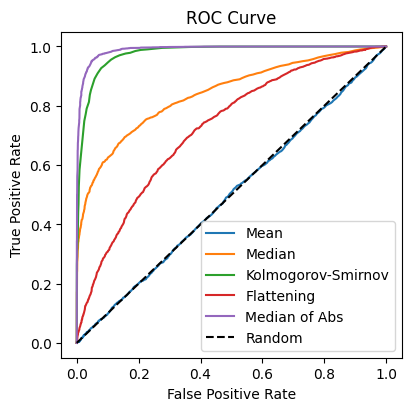
\includegraphics[width=7cm]{img/roc_curves.png}
\caption{ROC curves for different test statistics on simulated distributions in the VLTI context with a companion of contrast $10^{-2}$.}
\label{fig:roc}
\end{figure}

\begin{figure}[H]
\centering
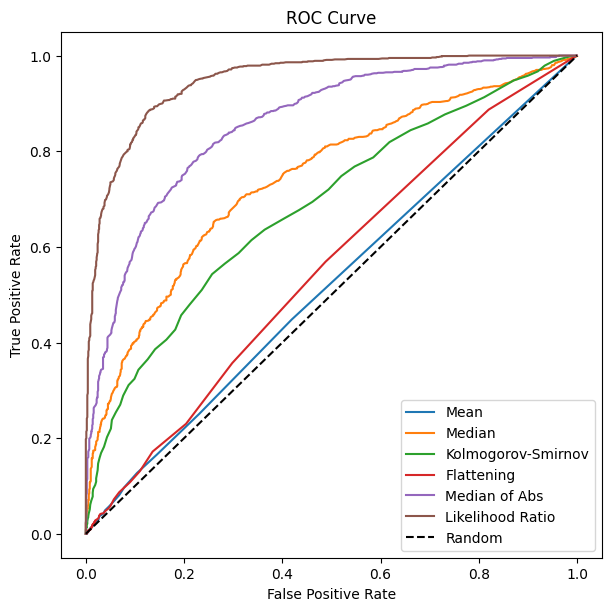
\includegraphics[width=7cm]{img/neyman_pearson.png}
\caption{ROC curves for different test statistics compared to the optimal Neyman-Pearson test, in the VLTI context with a companion of contrast $10^{-3}$.}
\label{fig:neyman-pearson}
\end{figure}

\hl{Results analysis}

\subsection{P-value analysis}

\dm{Attention Fig.4 c'est faux : ce ne sont pas les p-valeurs car les p-valeurs ne dépendent pas d'un seuil, seulement des données.}

P-values provide a confidence measure for rejecting the null hypothesis. A P-value less than 0.05 is generally considered significant. \dm{Non ça ça dépend des applications. Donne la définition précise de la p-valeur tout de suite, comme ça on sait de quoi on parle. }\\


\begin{figure}[H]
\centering
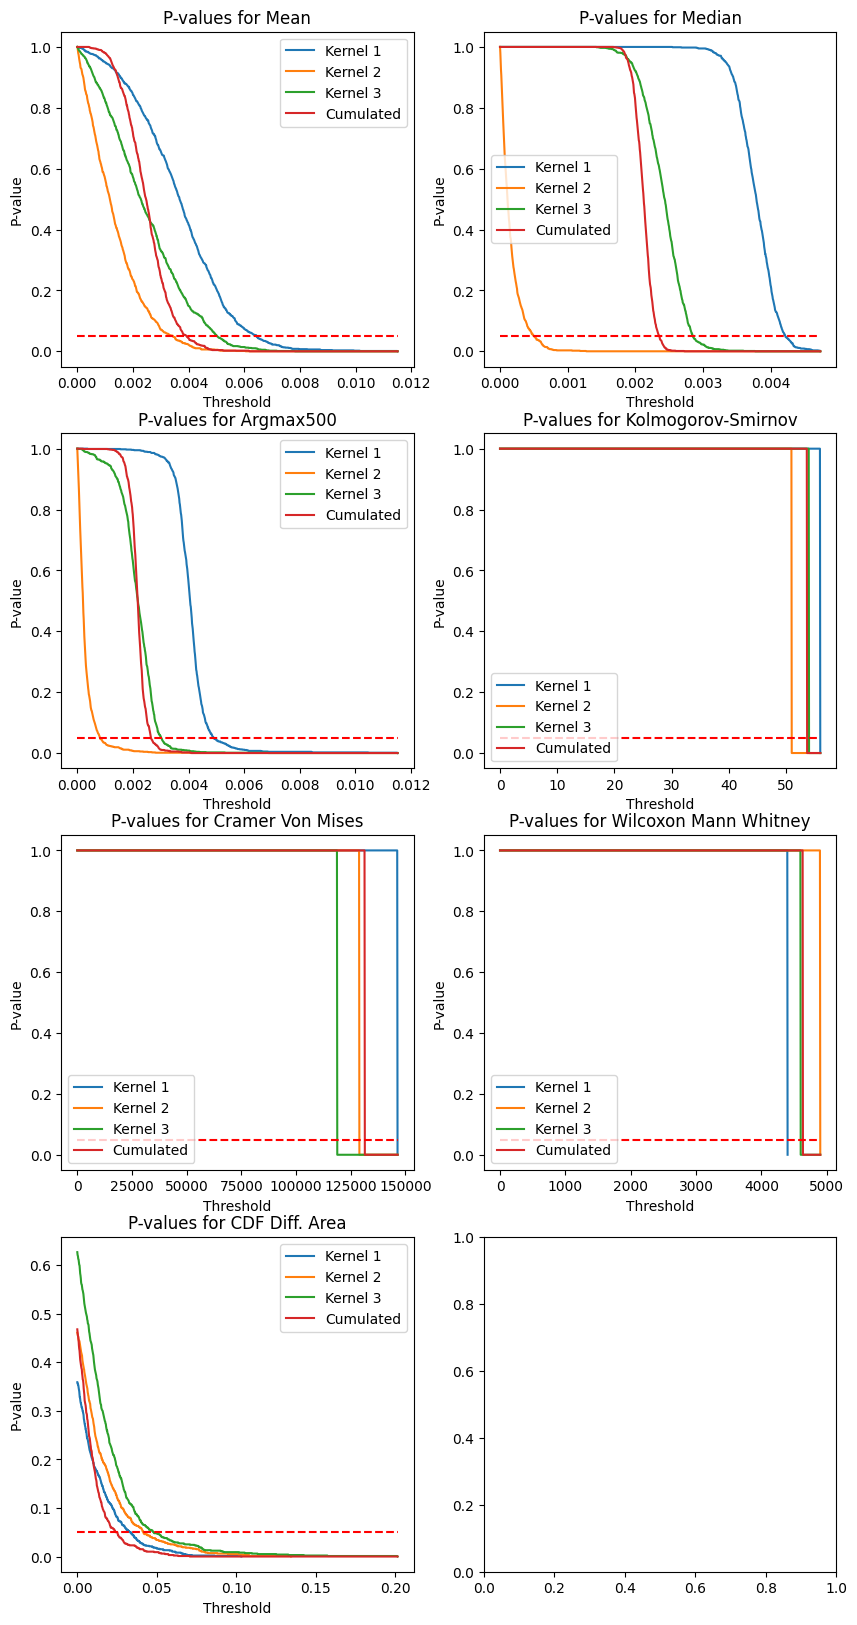
\includegraphics[width=10cm]{img/p-values.png}
\caption{Evolution of P-values as a function of threshold for different test statistics. The red dashed line indicates the significance threshold at 0.05. \hl{Plot to redo to focus on a single Kernel (+ bug corrections)} \dm{Oui. On peut par exemple montrer la calibration théorique p-valeur(stat de test - pas seuil !) et comparer à la calibration empirique pour chaque test }}


\label{fig:pvalues}
\end{figure}

\hl{Results analysis}

%--------------------------------------------------------------------

\section{Discussion}

\subsection{Comparative performance of tests}

\hl{ToDo}

\subsection{Noise sensitivity}

\hl{ToDo}


%-----------------------------------------------------------------

\section{Conclusions}

\hl{ToDo}

\bibliographystyle{alpha}
\bibliography{sample}

\end{document}